\begin{figure}[H]
\centering
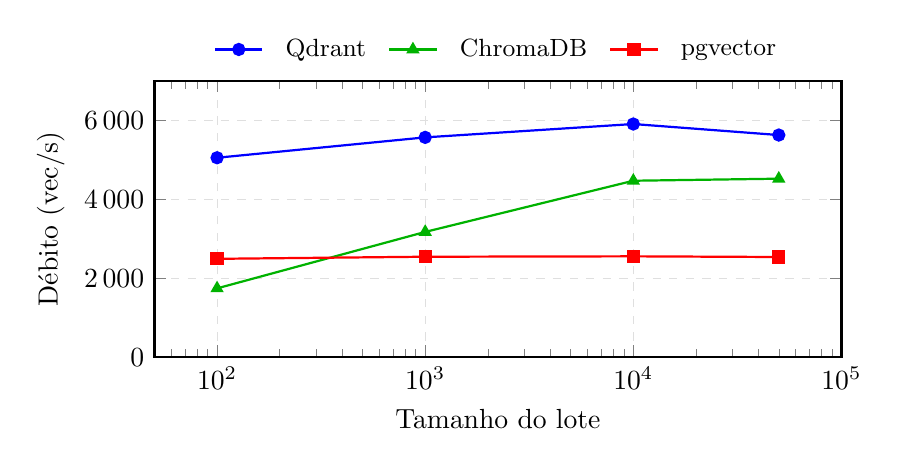
\begin{tikzpicture}
\begin{axis}[
    width=0.85\textwidth,
    height=0.42\textwidth,
    xlabel={Tamanho do lote},
    ylabel={Débito (vec/s)},
    xmode=log,
    log basis x={10},
    xmin=50, xmax=100000,
    ymin=0, ymax=7000,
    legend columns=3,
    legend style={at={(0.5,1.03)}, anchor=south, font=\small, draw=none, /tikz/column sep=6pt},
    /pgf/number format/1000 sep={\,},
    grid=major,
    grid style={dashed, gray!25},
    thick,
    mark options={solid}
]
\addplot[color=blue, mark=*] coordinates {
    (100, 5048) (1000, 5564) (10000, 5902) (50000, 5623)
};
\addlegendentry{Qdrant}
\addplot[color=green!70!black, mark=triangle*] coordinates {
    (100, 1741) (1000, 3170) (10000, 4466) (50000, 4518)
};
\addlegendentry{ChromaDB}
\addplot[color=red, mark=square*] coordinates {
    (100, 2489) (1000, 2542) (10000, 2552) (50000, 2535)
};
\addlegendentry{pgvector}
\end{axis}
\end{tikzpicture}
\caption{Débito de inserção em lote para a \textbf{Similaridade de Cosseno}, medido até a coleção estar pronta a pesquisar (mediana de 3 réplicas). Nos lotes acima de \num{10000} (Qdrant) e de \num{5461} (ChromaDB), os vetores são enviados em pedidos de tamanho máximo.}
\label{fig:batch_throughput_cosine}
\end{figure}
